%#BIBTEX jbibtex main
%%%%%%%%%%%%%%%%%%%%%%%%%%%%%%%%%%%%%%%%%%%%%%%%%%%%%%%%%%%%%%%%%%%%%%%%
%%
%% template.tex
%% このサンプルは,LaTeX-2e 専用です。
%%
%% Change Lgo
%% 2010-04-19 Yasuhiro Sugimoto <yas@mech.eng.osaka-u.ac.jp>
%% * 大須賀・石川研研究会資料用に修正
%%
%% 2018-1-1 Keisuke Naniwa <naniwa@es.hokudai.ac.jp>
%% * 大須賀・杉本研研究会資料用に修正
%%   osukaLab2018.styを使用することを前提にした記述とパッケージに変更
%%  いくつかのべからず集を記載してあるので,熟読の上資料作成のこと(ここすら読んでないなら知らん)
%%
%%  $Id: template.tex,v 1.2 2000/01/12 08:18:03 ken Exp $
%%
%%%%%%%%%%%%%%%%%%%%%%%%%%%%%%%%%%%%%%%%%%%%%%%%%%%%%%%%%%%%%%%%%%%%%%%%
%\RequirePackage[l2tabu, orthodox]{nag}%おまじない

\documentclass[a4j]{jsarticle}
\usepackage{soturonyoukou}%使用前にstyファイル内を一度目を通しておくこと
\usepackage{epic,eepic}
\usepackage[dvipdfmx]{graphicx}
\usepackage{amsmath}	% required for `\align' (yatex added)もし必要なパッケージがインクルードされてない場合,こんな感じでやてふが自動で入れてくれます(ただし^C^Bでやった場合だけ.みんな^C^B使ってるよね・・・?)
\usepackage[all, warning]{onlyamsmath}
\usepackage{epsfig} % このパッケージは使わずに画像の形式はPDFを使いましょう
%写真はjpg,スクショはpng,グラフやイラストはpdfで
%matlabでのグラフ出力については別で
\usepackage{siunitx} %単位や数値が綺麗に入ります
%\usepackage{times} % これもう古いのでtxfonts使おね
\usepackage{txfonts} %綺麗なtimesフォント系への切り替え
\usepackage{amssymb}
\numberwithin{equation}{section}%式がたくさん出る人はこちらをどうぞ,3章の5式目とかがeq.(3.5)とかになります
\pagestyle{empty}
\newcommand{\argmax}{\mathop{\rm arg~max}\limits}
\newcommand{\argmin}{\mathop{\rm arg~min}\limits}

\setlength\intextsep{3pt}
\setlength\textfloatsep{3pt}

\makeatletter
\def\@cite#1{[#1]}
\makeatother



%\headding{大須賀・杉本研 研究会資料}
% 和文題名

\title{不安定物体を協調支持・搬送可能な群ロボット:CarryBotsの開発}


% 英文題名 英文題名とか,英文著者名入れたい時はosukalab2018.styの中身をいじってちょ
%\etitle{p\LaTeX-Style file for Osuka-Sugimoto Lab. Meeting}
% 著者の和文名
\author{YONG\ WEI JIE}
% 著者の英文名
%\engauthor{
%     Keisuke NANIWA
%}
% 英文の概要
%\abstract{Please write your English abstract here.}
% キーワード
%\keywords{研究会資料,大須賀・杉本研,大阪大学}
%
\usepackage{setspace}
\begin{document}
\maketitle
\thispagestyle{empty}

%
\setstretch{0.8}

\section{緒言}
\labsec{introduction}
近年,複数の移動ロボットから構成される群ロボットシステムの研究が進められている.
群ロボットを活かした応用先として,環境センシング,モニタリングなどがある.
その中で,本研究では群ロボットによる協調運搬に着目する.
群ロボットの協調運搬として,把持機構を利用し物体を掴んで運搬する「掴む方法」とロボットの体のみで物体を押すことで協調運搬する「押す方法」がある~\cite{swarmBot,push-only2}.
掴む方法は,ロボットに搭載された把持機構で物体を掴むので,押す方法より安定に運搬できるが,物体の認識と把持機構の制御が必要である.
一方,押す方法は倒れやすい不安定な物体が運搬できないという課題がある.
そこで本研究では,対象物体の重心付近まで乗り上げることで把持機構なしで倒れやすい不安定な物体を運搬可能なロボット群を提案する.
そして,製作したロボットを用いて他のロボットに乗り上げる実験を行った.
さらに,ロボットの段数および前進力の制御を変更し,物体の安定化性能の検証実験を行った.
%~~~~~~~~~~~~~~~~~~~~~~~~~~~~~~~~~~~~~~~~~~~~~~~~~~~~~~~~~~~~~~~~~~~~~~~~
% %cant fit it....
\section{システムのモデリング}
本章では,提案する不安定物体を支持可能な群ロボットシステムとシステムのモデリングについて説明する.
提案システムを実現するために,ロボット群が物体を支持する支持部とシステム全体を移動する移動部に分ける必要がある.
また,ロボットの台数は限られているので,支持部のロボットの台数が多いほど,物体を安定に支持できるが,移動部に負担がかかるため,全体の移動速度が遅くなることが考えられる.一方,移動部に関しては,ロボットが多いほど,全体の速度は速いが,支持部のロボットが少ないため,物体が倒れる可能性がある.
本稿ではその前段階として,支持部のロボットが物体を支えるための条件を検討する.

提案システムのモデリングした図を\reffig{modeling}に示す.
\begin{figure}[b]
  \centering
  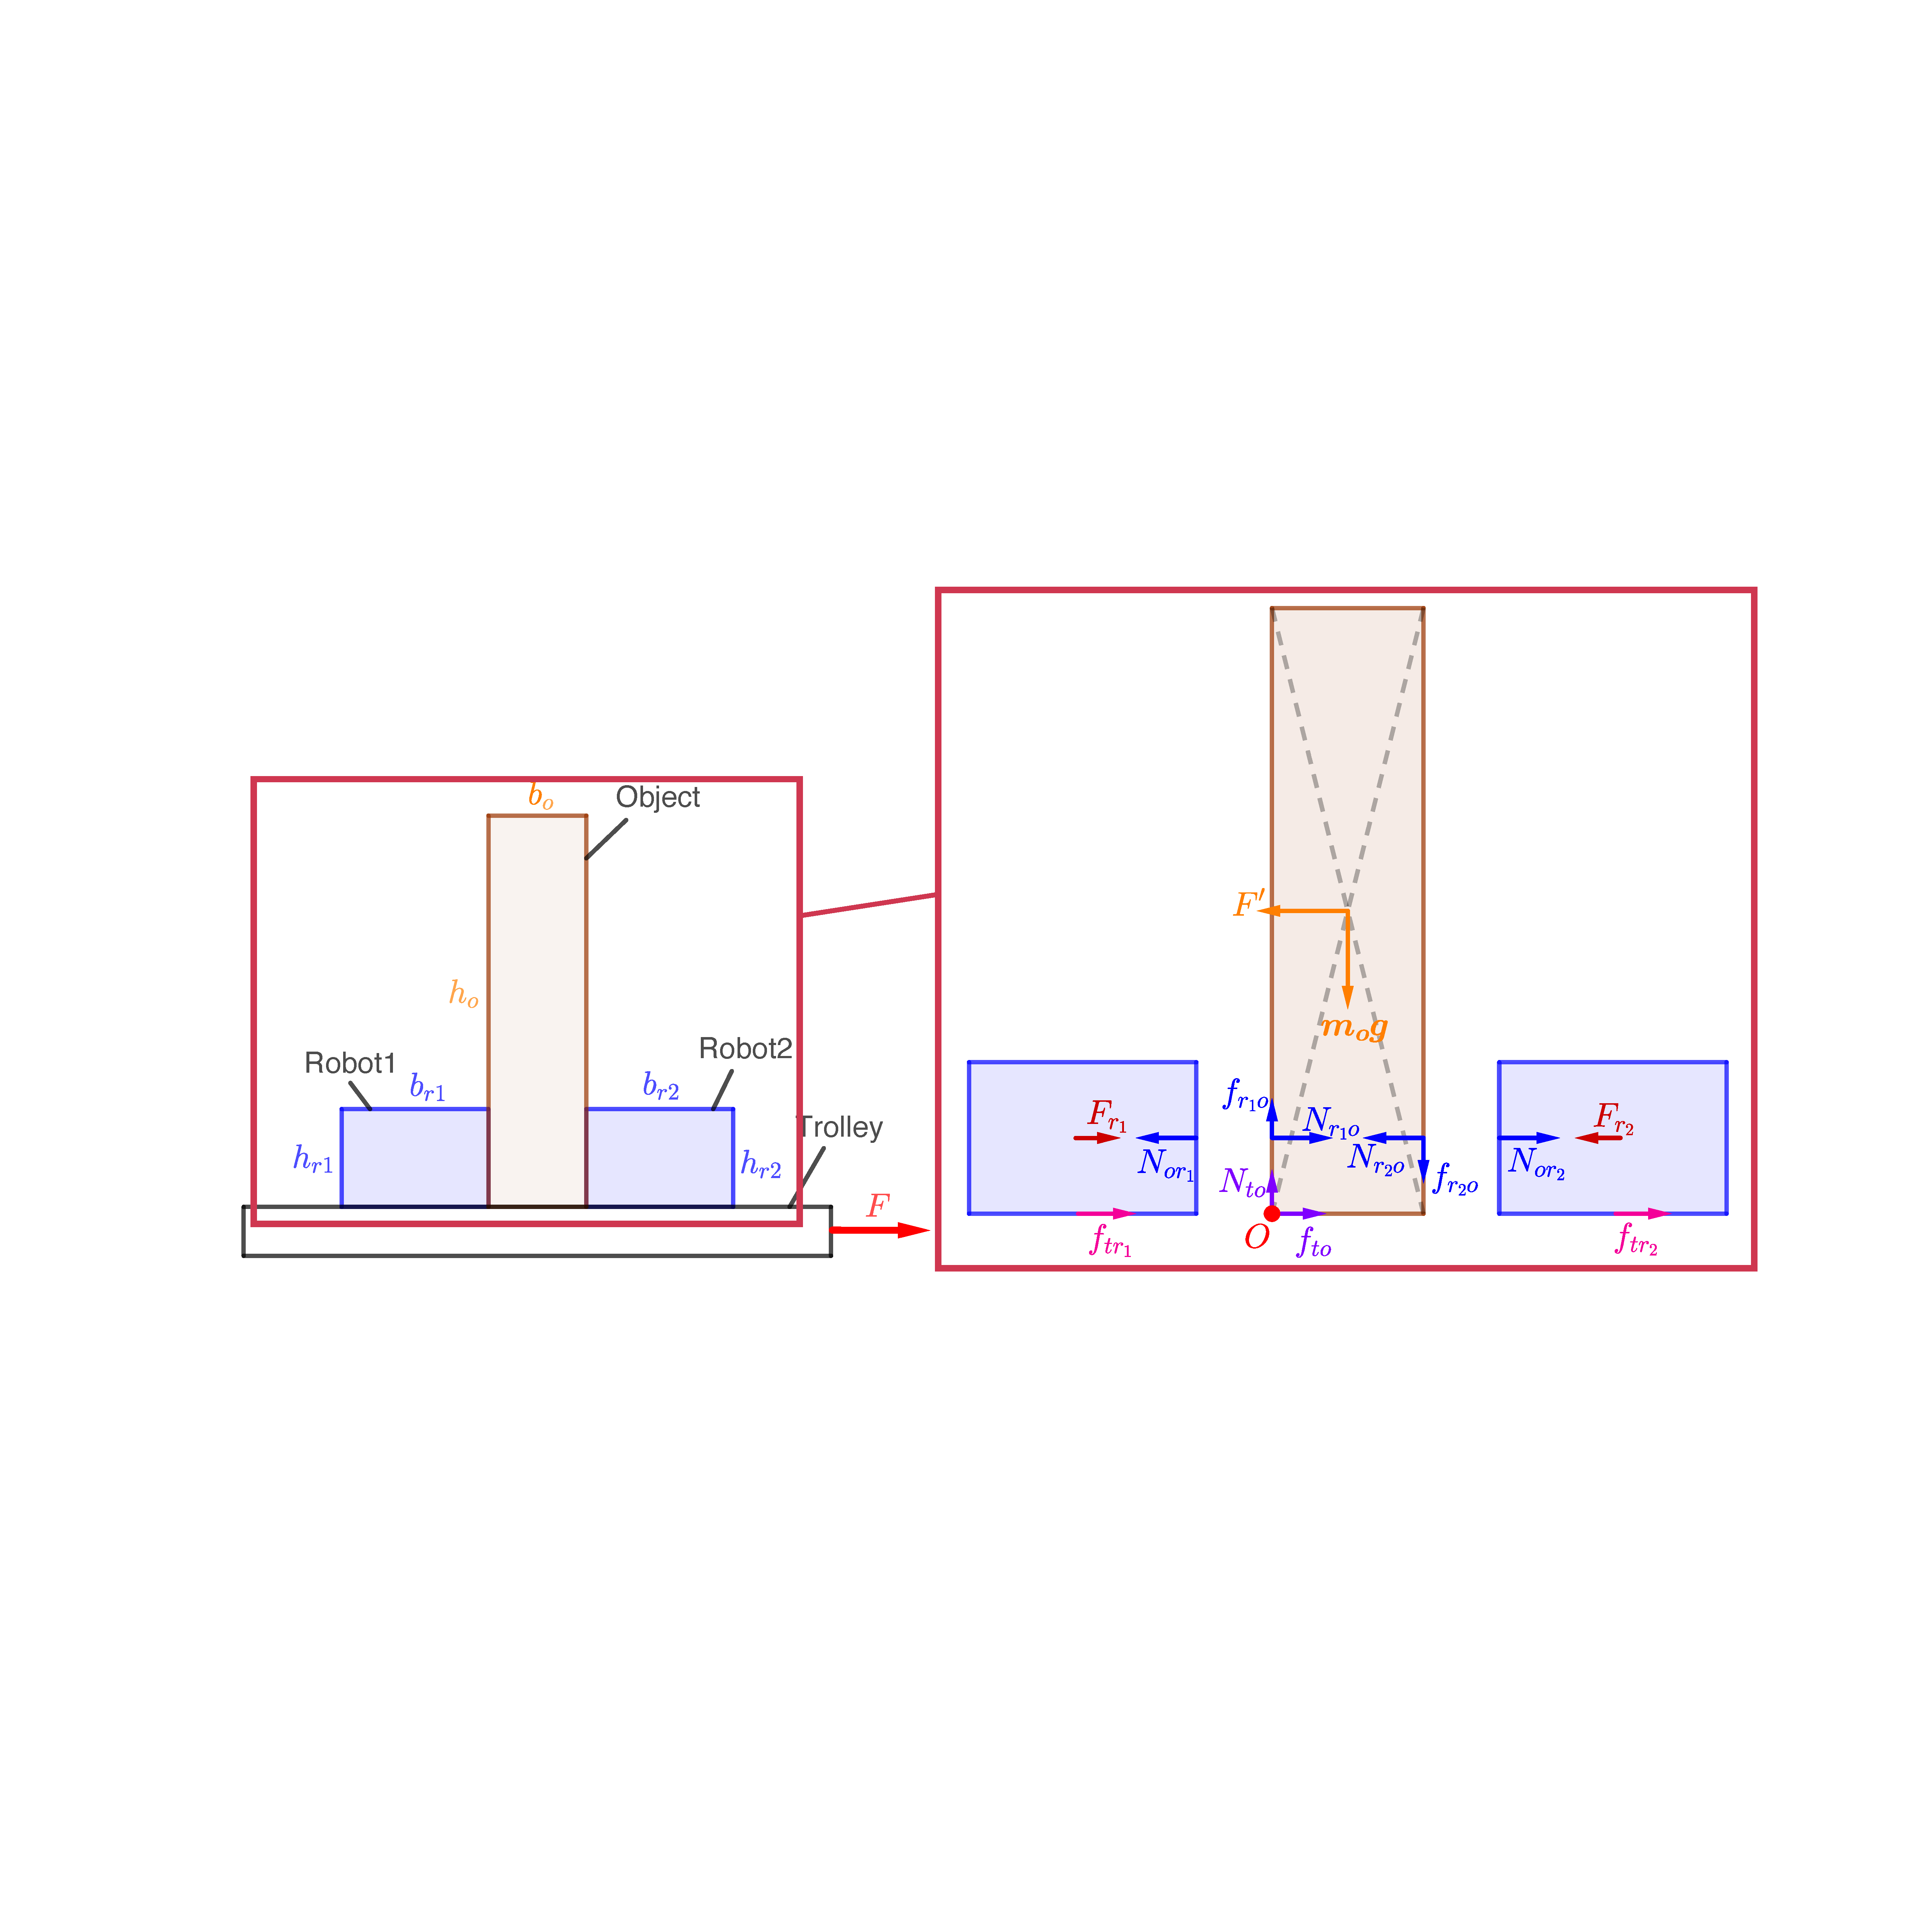
\includegraphics[width=0.9\columnwidth]{figures/modeling.pdf}
  \caption{Simplified model, free body diagram}
  \label{fig:modeling}
\end{figure}
また,モデリングに使用した変数を\reftab{model-parameter}に示す.
\begin{table}[tb]
\caption{Parameters of model}
\centering
\scalebox{0.7}{
\begin{tabular}{c|c}
\hline
Parameter & Description                   \\ \hline\hline
$b_o$       & Width of object              \\ \hline
$h_o$      & Height of object               \\ \hline
$h_r$      & Height of robot               \\ \hline
$m_o$     & Mass of object        \\ \hline
$f_{r_1 o}$       & Friction from robot1 acting on object                 \\ \hline
$f_{r_2 o}$ & Friction from robot2 acting on object                 \\ \hline
$f_{t o}$ & Friction from trolley acting on object                 \\ \hline
$N_{t o}$ & Normal force from trolley acting on object                 \\ \hline
$N_{r_1 o}$ & Normal force from robot1 acting on object                 \\ \hline
$N_{r_2 o}$ & Normal force from robot2 acting on object                 \\ \hline
$F_{r_1}$ & Force asserted by robot1                 \\ \hline
$F_{r_2}$ & Force asserted by robot2                 \\ \hline
\end{tabular}}
\label{tab:model-parameter}
\end{table}
次に,台車に大きな力$F$がかかっても物体は傾かないための条件を調べる.
点$O$まわりのモーメントの釣り合いから,以下の式が導かれる.
\[
    F<\frac{h_{r}}{h_{o}}\left(F_{r_{1}}-F_{r_{2}}+f_{t{r_1}}+f_{t{r_2}}\right)+\frac{b_{o}}{h_{o}}\left(m_{o} g+2 f_{r_2 o}\right)
\]
上式より,右辺を大きくすることで,物体をより安定に運べる.
今回,ロボットと台車の間の摩擦$f_{t{r_1}},f_{t{r_2}}$を大きくすることとロボットに前進力$F_{r_{1}},F_{r_{2}}$をかけることに注目した.
\section{CarryBotsの開発}
本章では,製作したロボットの概要について述べる.

\subsection{ロボットの概要}
前章で述べた式から,上下のロボット間の摩擦を上げることに着目する.
また,他のロボットに乗り上げることを実現する機構として,
\reffig{rack-pinion}に示すラックレール・ピニオン車輪構造を用いた.
さらに,ピニオン車輪の歯先に滑りにくい,軟質樹脂製パッドをつけ,車輪のグリップを高める.
そして,ロボットが物体の姿勢を検知するためのセンサとして,\reffig{limit-switch}に示すようにリミットスイッチを採用した.
このラックレール,ピニオン車輪と物体の姿勢を検知するセンサを用いて製作したロボットを\reffig{carrybot}に示す.
使用するモータは一つのみで,ギアを通じて車軸へ動力を伝達する.

\begin{figure}[tb]
  \begin{minipage}[b]{0.6\columnwidth}
  \centering
  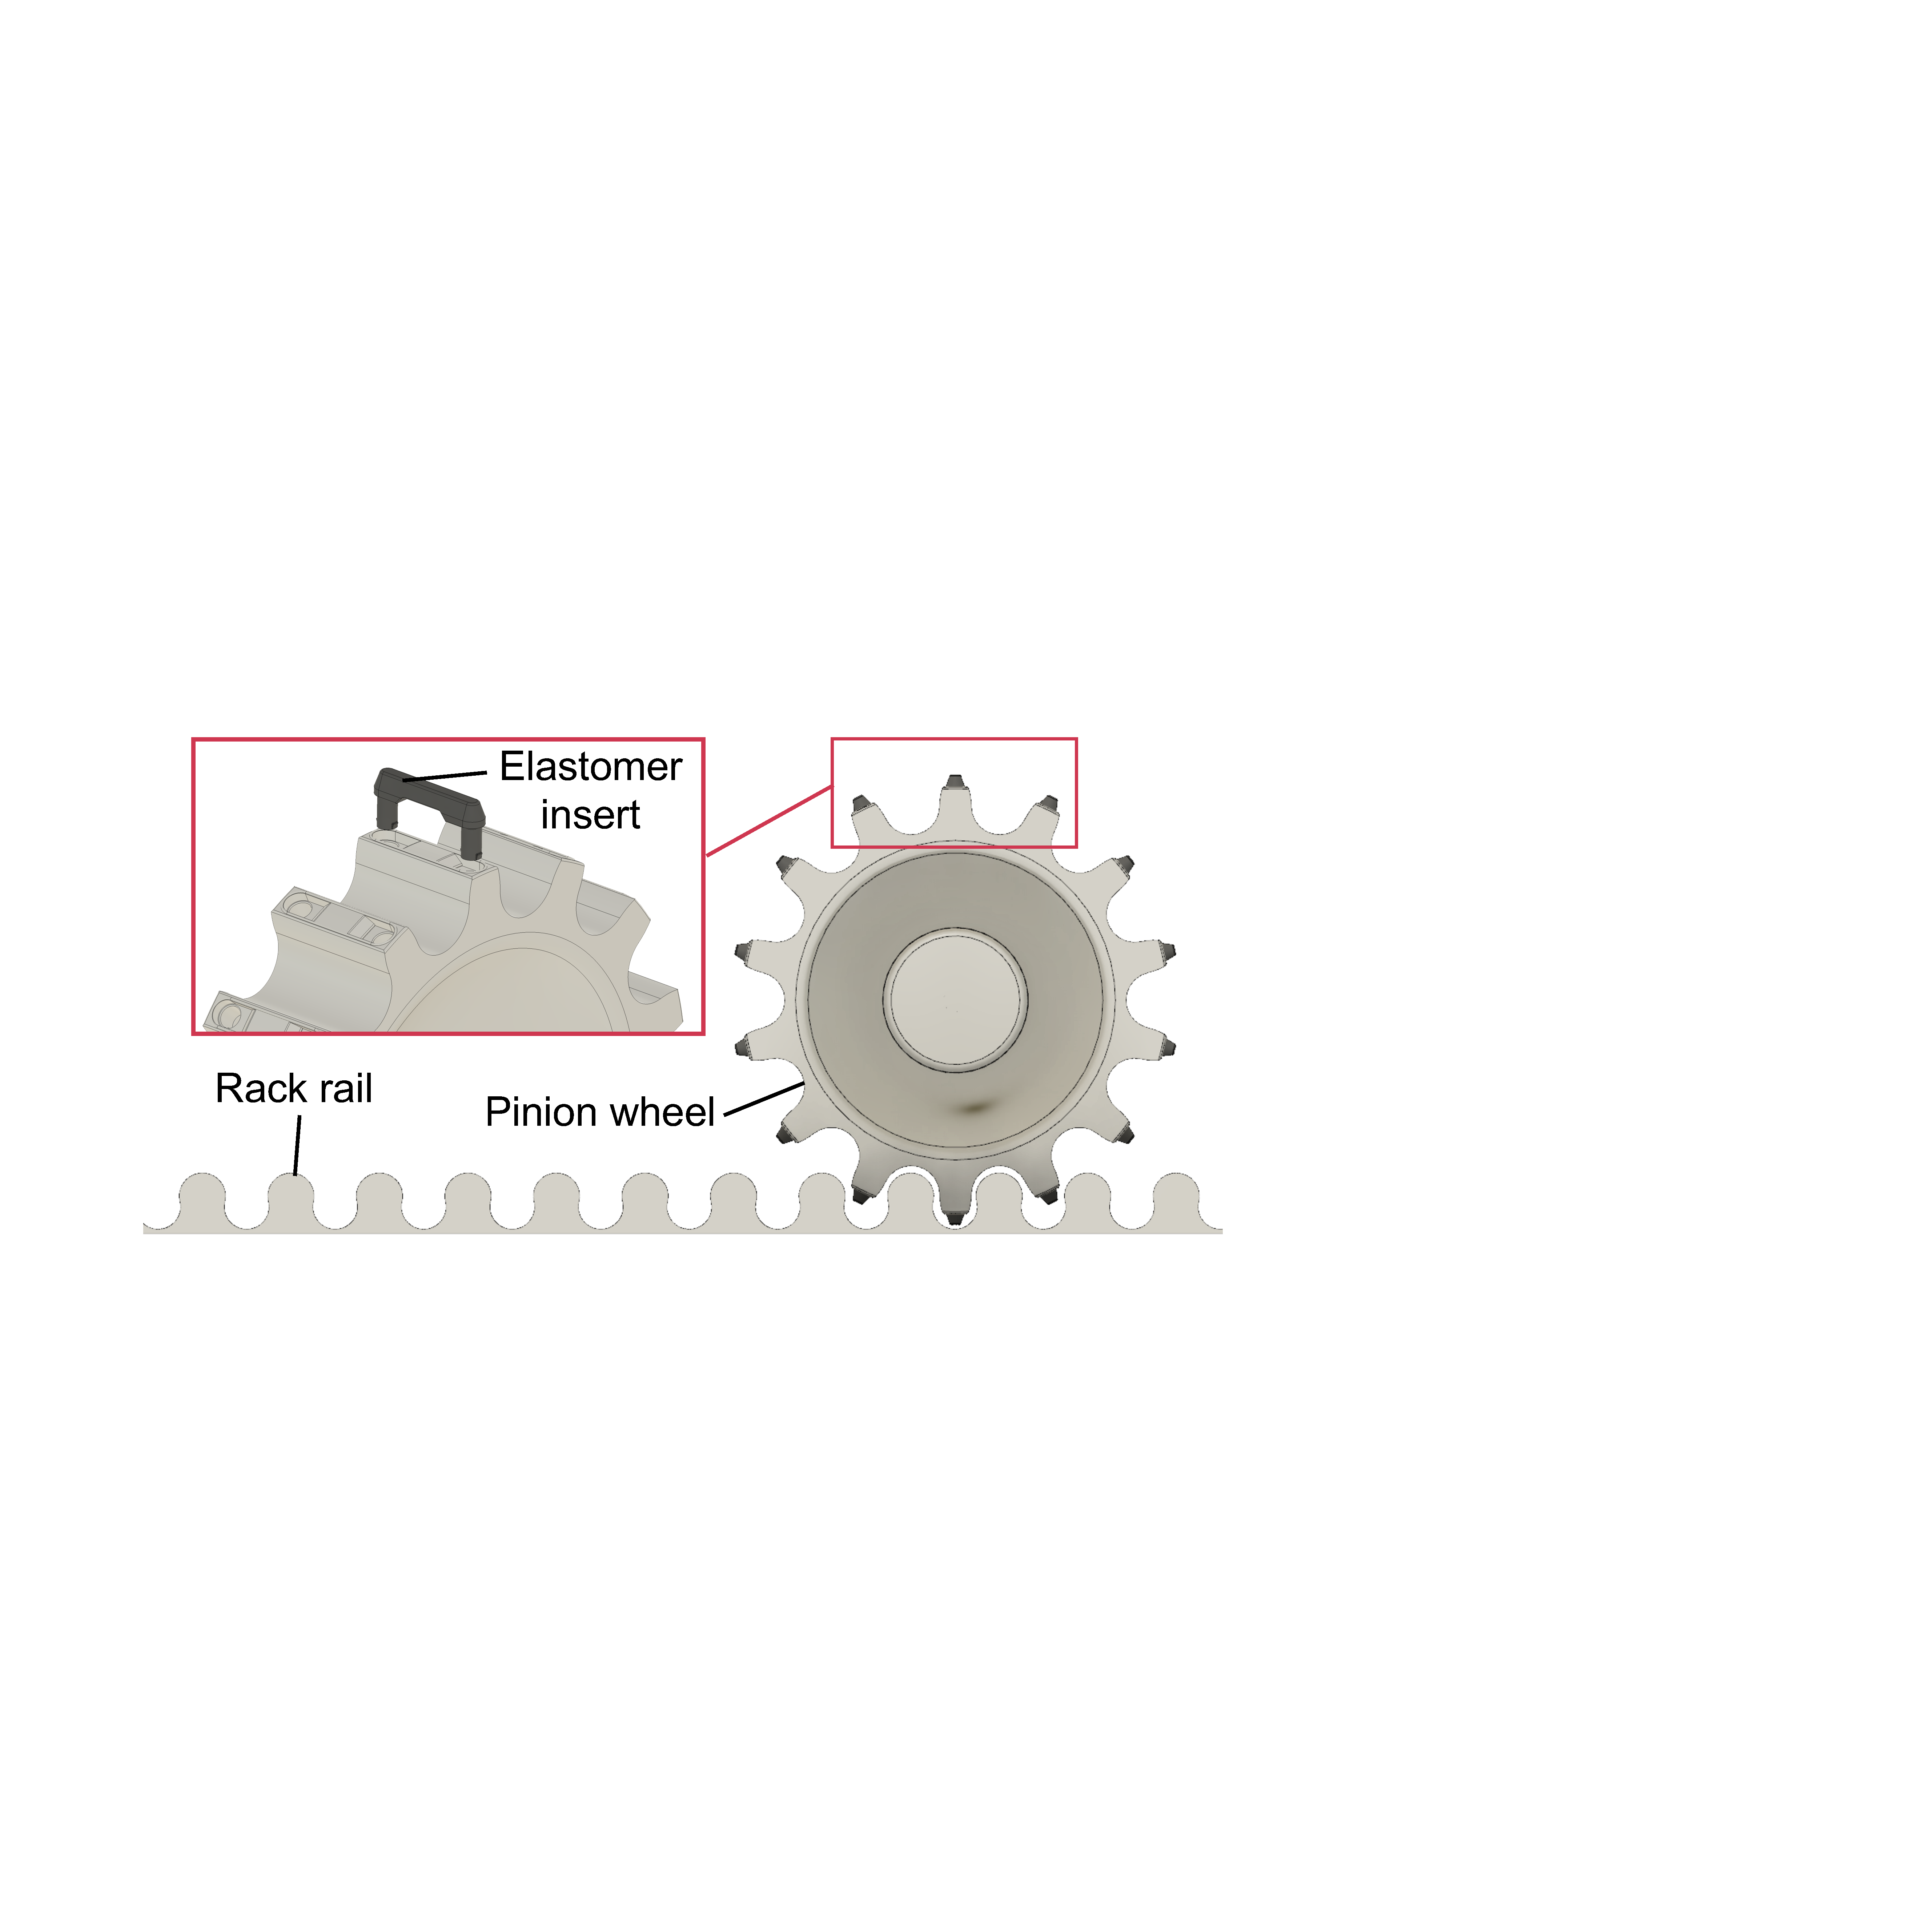
\includegraphics[width=0.95\columnwidth]{figures/rack-pinion.pdf}
  \subcaption{Rack-rail \& pinion-wheel}
  \label{fig:rack-pinion}
 \end{minipage}%
 \begin{minipage}[b]{0.4\columnwidth}
  \centering
  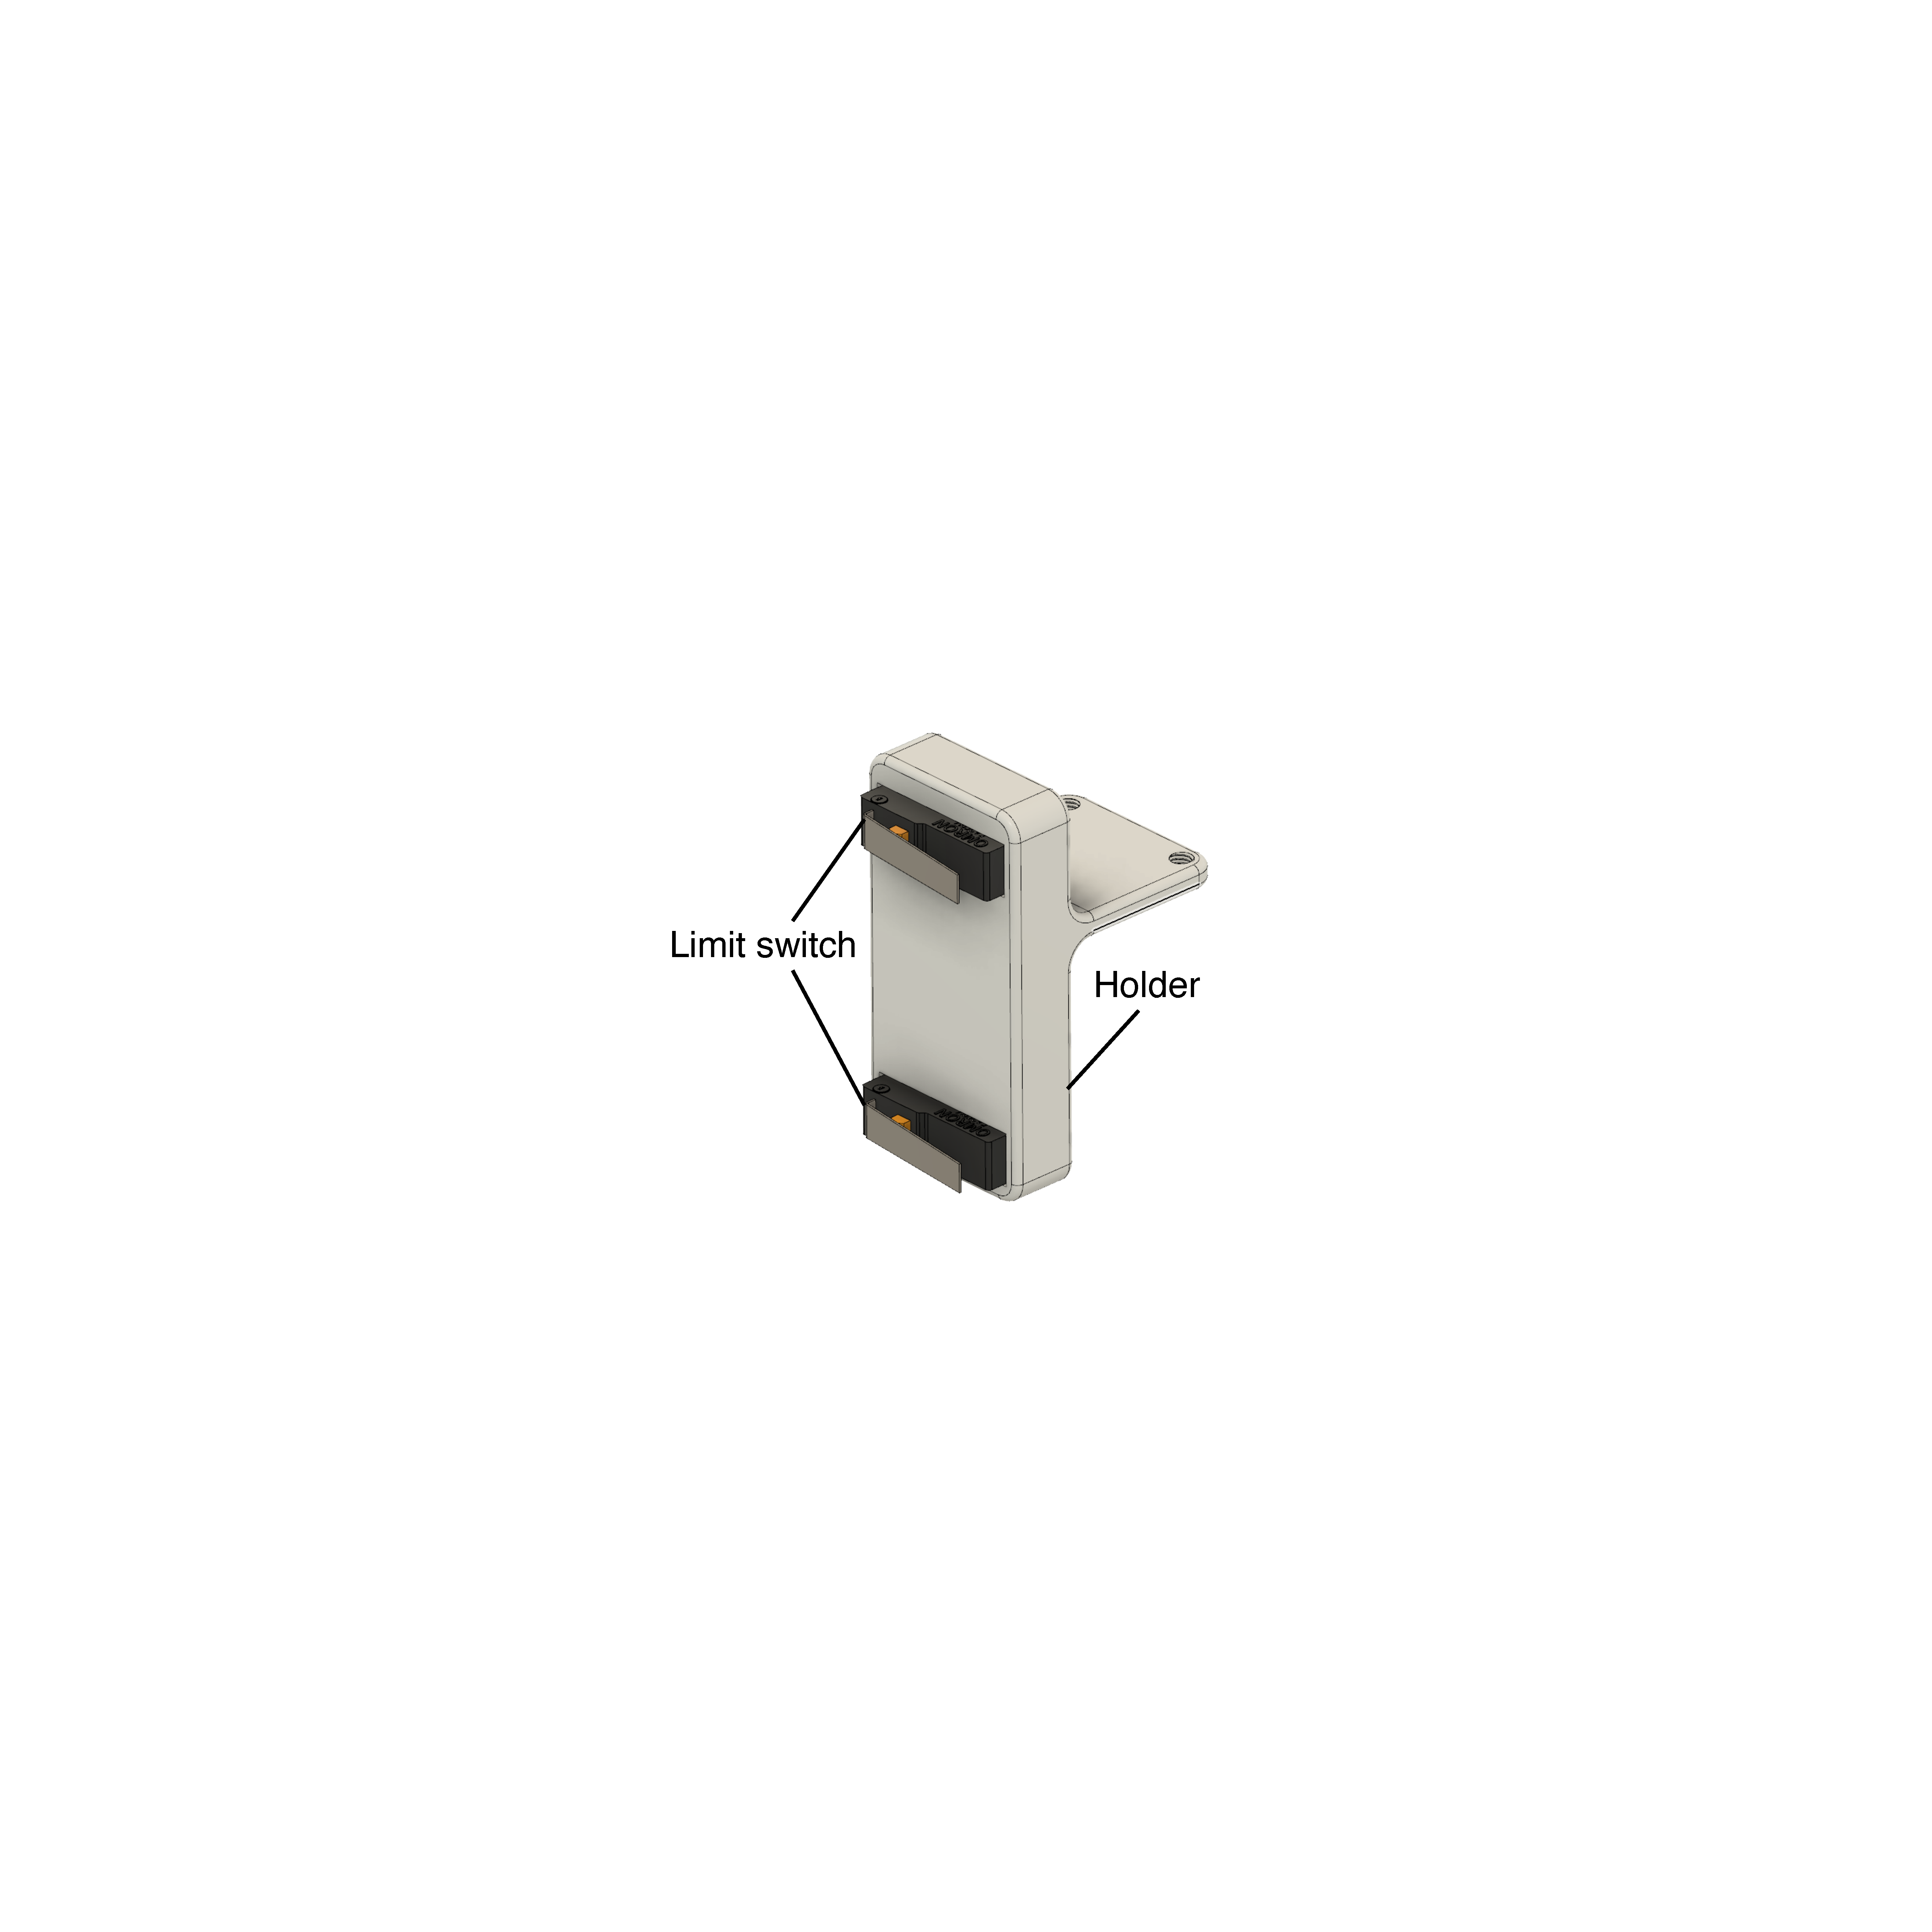
\includegraphics[width=0.95\columnwidth]{figures/limit-switch.pdf}
  \subcaption{Posture detector}
  \label{fig:limit-switch}
 \end{minipage}
 \caption{Proposed mechanism}
 \label{fig:mechanism}
\end{figure}
\begin{figure}[tb]
  \begin{minipage}[b]{0.5\columnwidth}
  \centering
  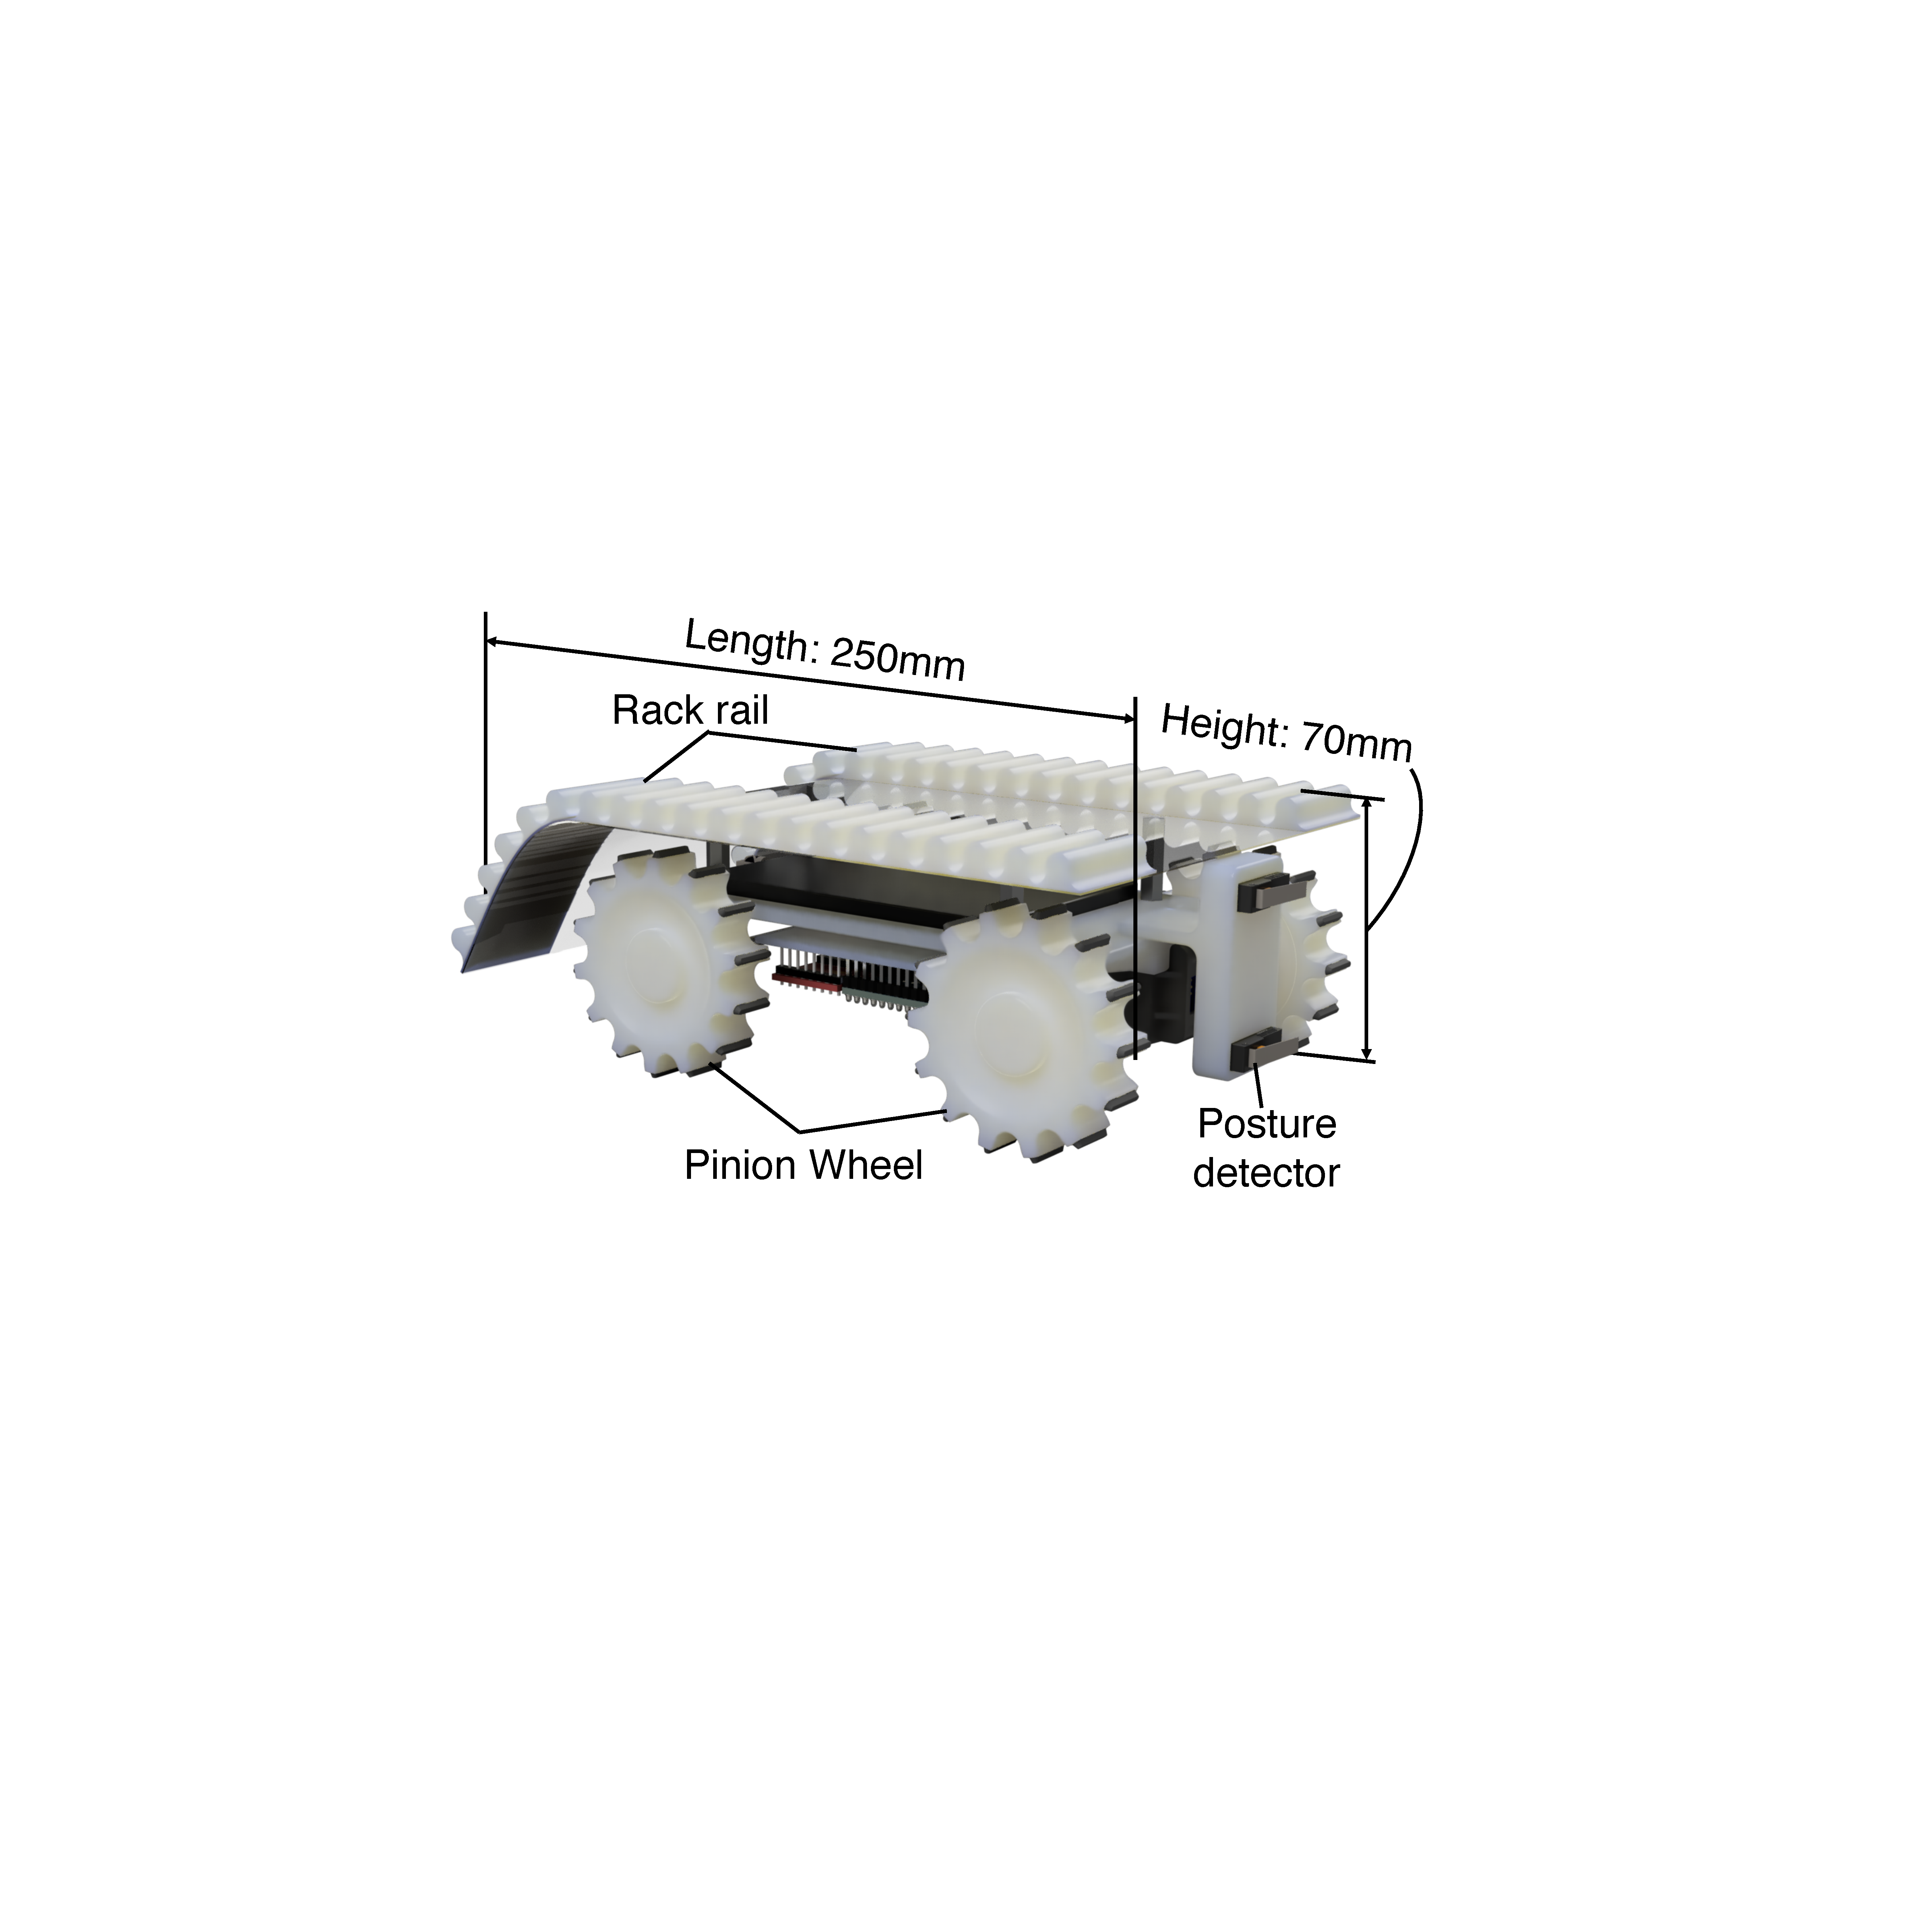
\includegraphics[width=0.9\columnwidth]{figures/carrybot-diagonal.pdf}
  \subcaption{Diagonal view}
  \label{fig:diagonal}
 \end{minipage}%
 \begin{minipage}[b]{0.5\columnwidth}
  \centering
  \includegraphics[width=0.9\columnwidth]{figures/carrybot-bottom.pdf}
  \subcaption{Bottom view}
  \label{fig:bottom}
 \end{minipage}
 \caption{Mechanical structure of the robot}
 \label{fig:carrybot}
\end{figure}

\section{実機実験}
% \labsec{experiment}
本章では製作したロボットを用いて行った実機実験について述べる.

\subsection{乗り上げる動作の検証}
ロボットが他のロボットに乗り上げることが実現できるかどうかを実機検証した.
\reffig{climb}から,ロボットが3段まで乗り上げられることが確認できた.
\begin{figure}[tb]
  \centering
  \includegraphics[width=\columnwidth]{figures/climb.pdf}
  \caption{Experiment of climbing}
  \label{fig:climb}
\end{figure}

% \subsection*{牽引装置}
% 次に,移動ロボットが移動しているとき,支持部のロボットが物体を支持できるかどうかを確認した.
% ここからの実験は提案システムの移動部をロボットの代わりとして,紙を使用した.
% また,紙を一定力で引っ張るために,\reffig{pulling-mechanism}に示すような牽引装置を作成した.
% 牽引装置はTAMIYA社のキャタピラ車をワイヤで机に前進しないように固定し,安定化電源で一定の電圧をかける. このとき,クローラーが摩擦よって,紙を送り出し,紙の上に載せているものを一定速度で動かすことができる.
\begin{figure}[tb]
  \centering
  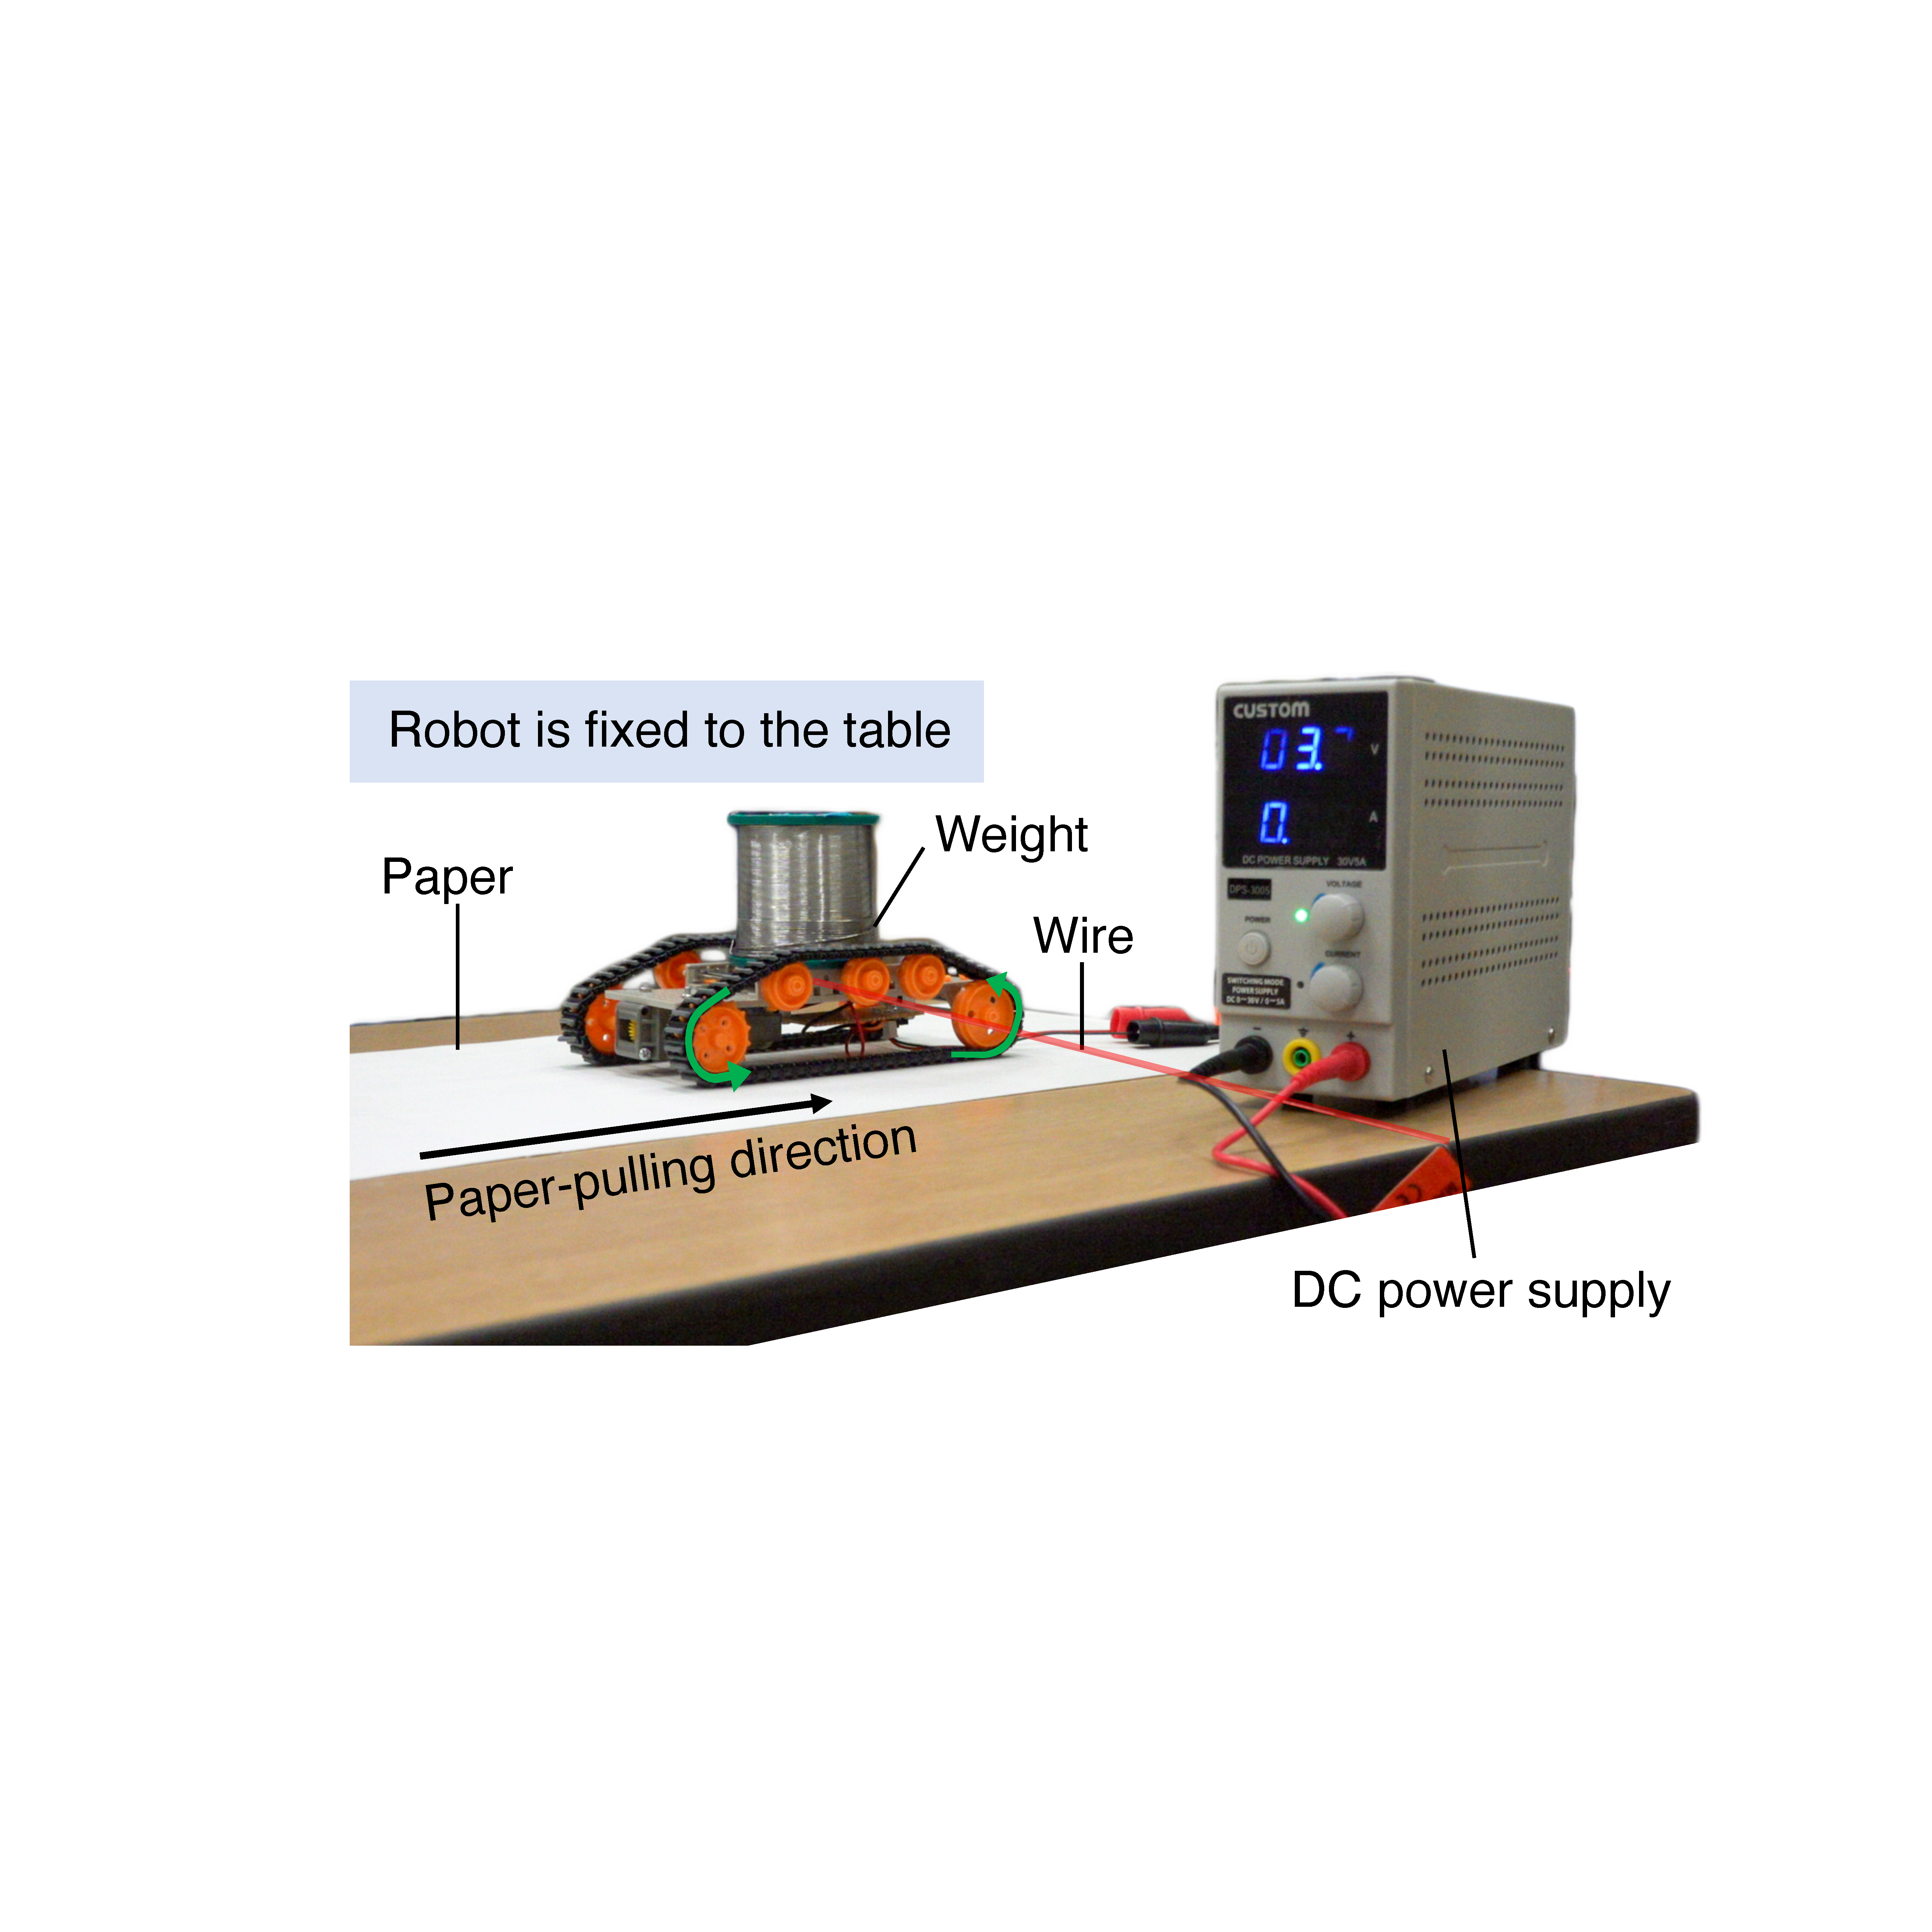
\includegraphics[width=0.85\columnwidth]{figures/pulling-mechanism.pdf}
  \caption{Pulling mechanism}
  \label{fig:pulling-mechanism}
\end{figure}
\subsection{段数の変更による物体の安定化性能に関する実験}
次に,移動ロボットが移動しているとき,支持部のロボットが物体を支持できるかどうかを確認した.
ここからの実験は提案システムの移動部をロボットの代わりとして,紙を使用した.
また,紙を一定力で引っ張るために,\reffig{pulling-mechanism}に示すような牽引装置を作成した.
牽引装置はTAMIYA社のキャタピラ車をワイヤで机に前進しないように固定し,安定化電源で一定の電圧をかける. このとき,クローラーが摩擦よって,紙を送り出し,紙の上に載せているものを一定速度で動かすことができる.

上述の牽引装置を利用し,搬送物体として本を立てて置いた.その両側にロボットを1段ずつと2段ずつ置き,牽引装置に6~Vの電圧を印加したときの安定化性能の比較を行った.
\reffig{1layer}から,1段の場合では紙を送り出すと物体は倒れた.
しかし,\reffig{2layer}から,2段の場合では紙を送り出してから止まるまで物体は初期姿勢を保つことができた.
その原因として,牽引装置の印加電圧が6~Vのとき,全体の加速度が大きいため,1段で支持する場合はロボットが滑ってしまい,物体を支持できなくなる.しかし,2段に増やすと,物体の重心近くで支持することと,2段のロボットが紙から滑りにくくなることによって,物体を支持し移動することができたと考えられる.
% よって,モデリングした式からロボットと物体の高さの比を大きくすることによって物体をより安定に支持することと一致する.
\begin{figure}[tb]
  \centering
  \includegraphics[width=\columnwidth]{figures/1layer.pdf}
  \caption{Experiment of supporting with 1 layer}
  \label{fig:1layer}
\end{figure}
\begin{figure}[tb]
  \centering
  \includegraphics[width=\columnwidth]{figures/2layers.pdf}
  \caption{Experiment of supporting with 2 layers}
  \label{fig:2layer}
\end{figure}

\subsection{制御による物体の安定化性能に関する実験}
製作したロボットの物体の姿勢を検知するセンサを利用し,物体の初期姿勢に戻そうとする制御をかけると,前節では物体を支持することができなかったロボットが1段の場合でも,物体を支持できるかを確認する実験を行った.
まず,\reffig{control-figure}に示すようにかける制御について述べる.\reffig{upright}より,センサの上下両方のスイッチが反応したとき,ロボットに対して物体は安定であると判断し,ロボットは前進しない.
しかし,\reffig{tilted}より,もし物体が右に傾いている場合,左のロボットに取り付けられたセンサは下のスイッチのみ反応する一方,右のロボットに取り付けられたセンサは上のスイッチのみ反応する.
このとき,右のロボットが左のロボットより大きい速度で物体を押し付けることで,物体の姿勢を保つと考える.
% よって,ロボット1とロボット2の前進力を加えることにより物体をより安定に支持することと一致する.
\begin{figure}[tb]
  \begin{minipage}{\hsize}
  \centering
  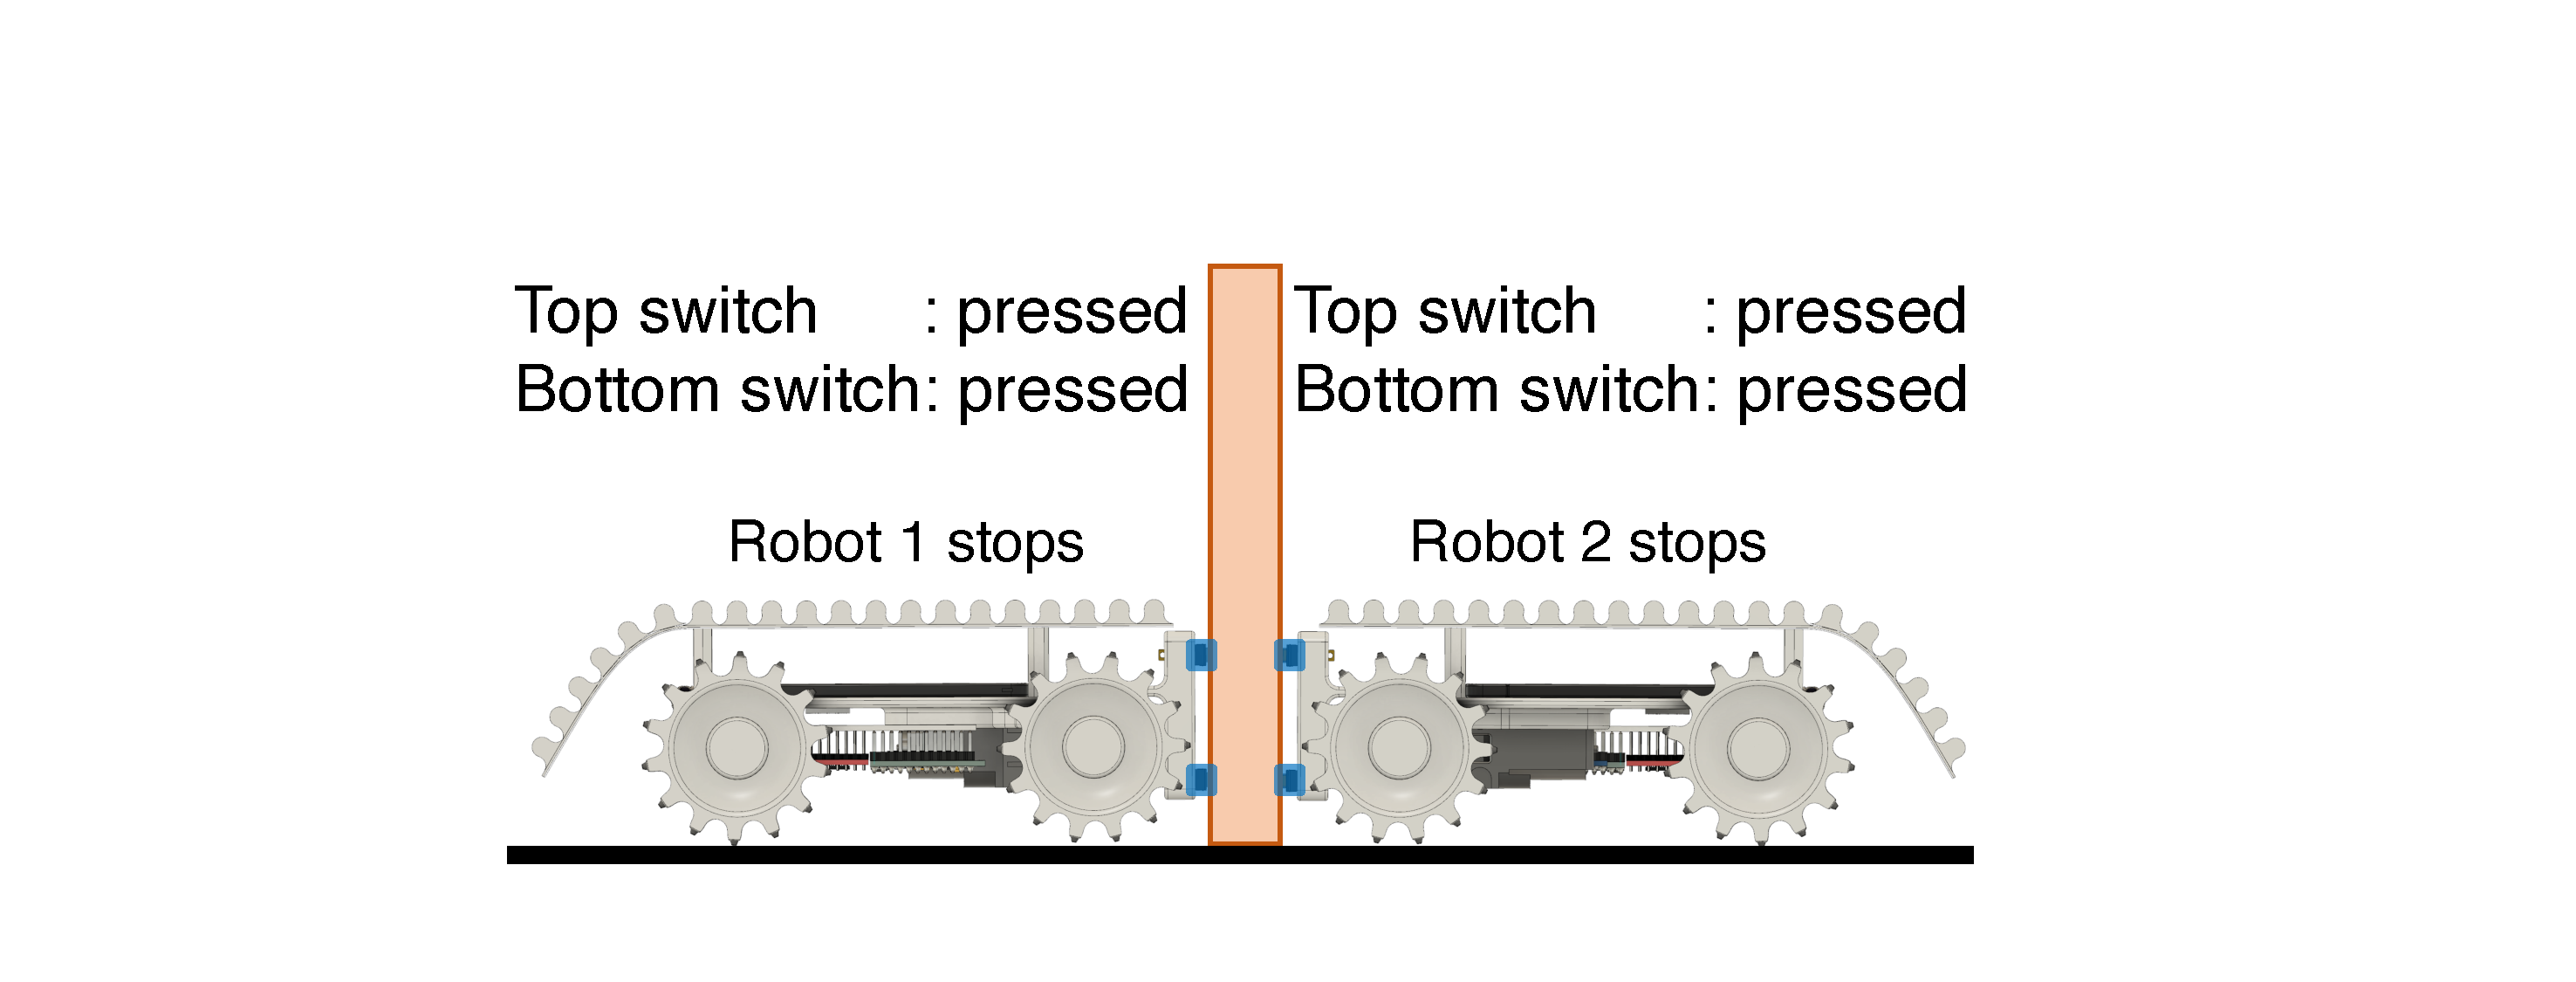
\includegraphics[width=0.65\columnwidth]{figures/control-upright-v3.pdf}
  \subcaption{Object is upright}
  \label{fig:upright}
 \end{minipage}\\
 \begin{minipage}{\hsize}
  \centering
  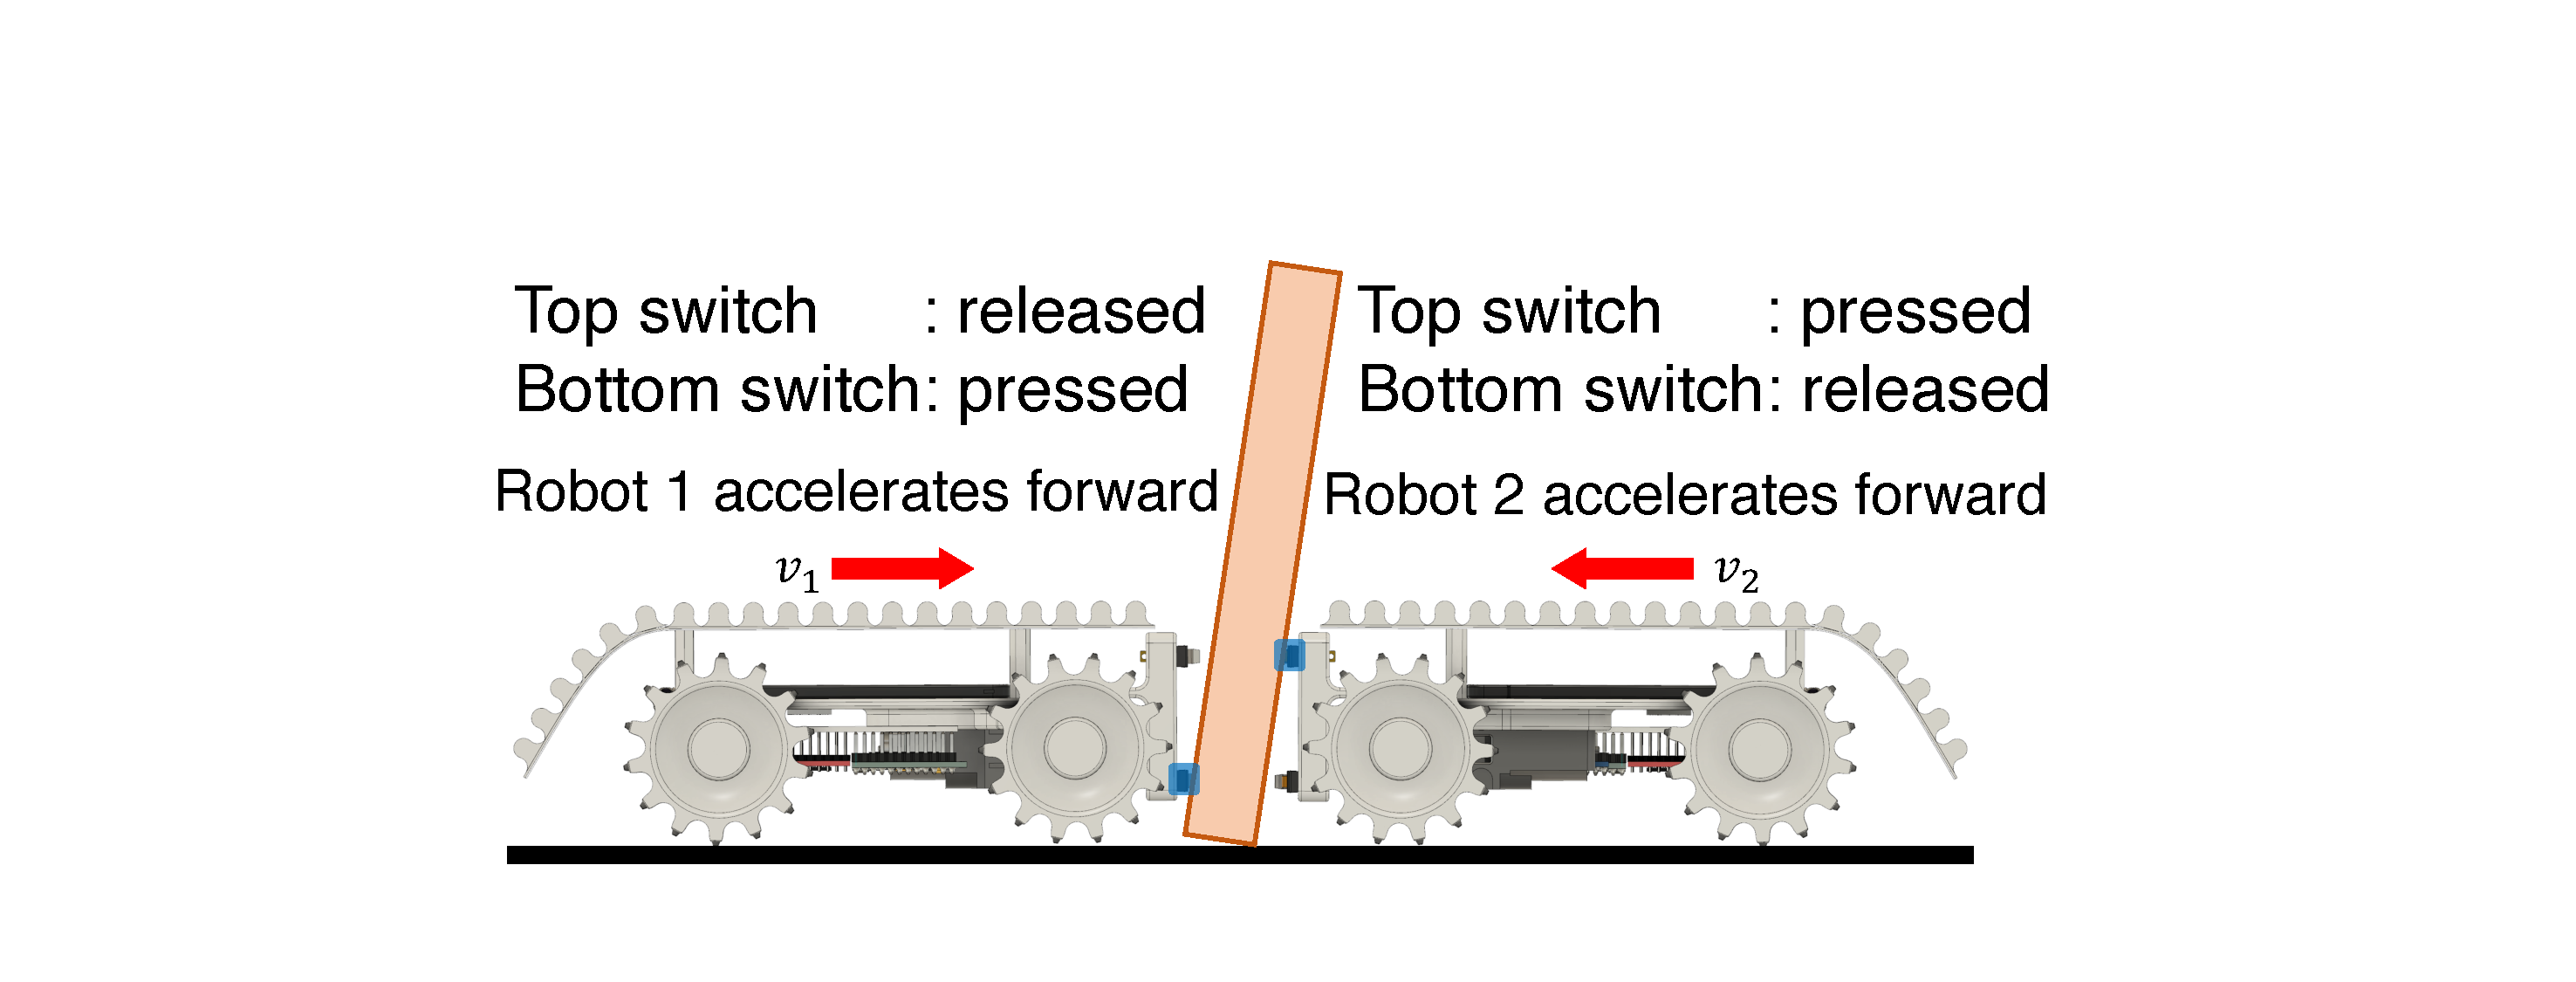
\includegraphics[width=0.65\columnwidth]{figures/control-tilted-v3.pdf}
  \subcaption{Object is tilted}
  \label{fig:tilted}
 \end{minipage}
 \caption{Overview of control system}
 \label{fig:control-figure}
\end{figure}
\reffig{control}より,紙を送り出した瞬間,ロボットはまだ反応していないときに,物体は傾いた.
しかし,その後はロボットのセンサが反応するため,ロボットが物体を初期姿勢に戻そうとする.
これによって全体が止まるまで物体を支持できることが確認できた.
\begin{figure}[tb]
  \centering
  \includegraphics[width=\columnwidth]{figures/1layer-control.pdf}
  \caption{Experiment of applying control}
  \label{fig:control}
\end{figure}
\begin{figure}[tb]
  \centering
  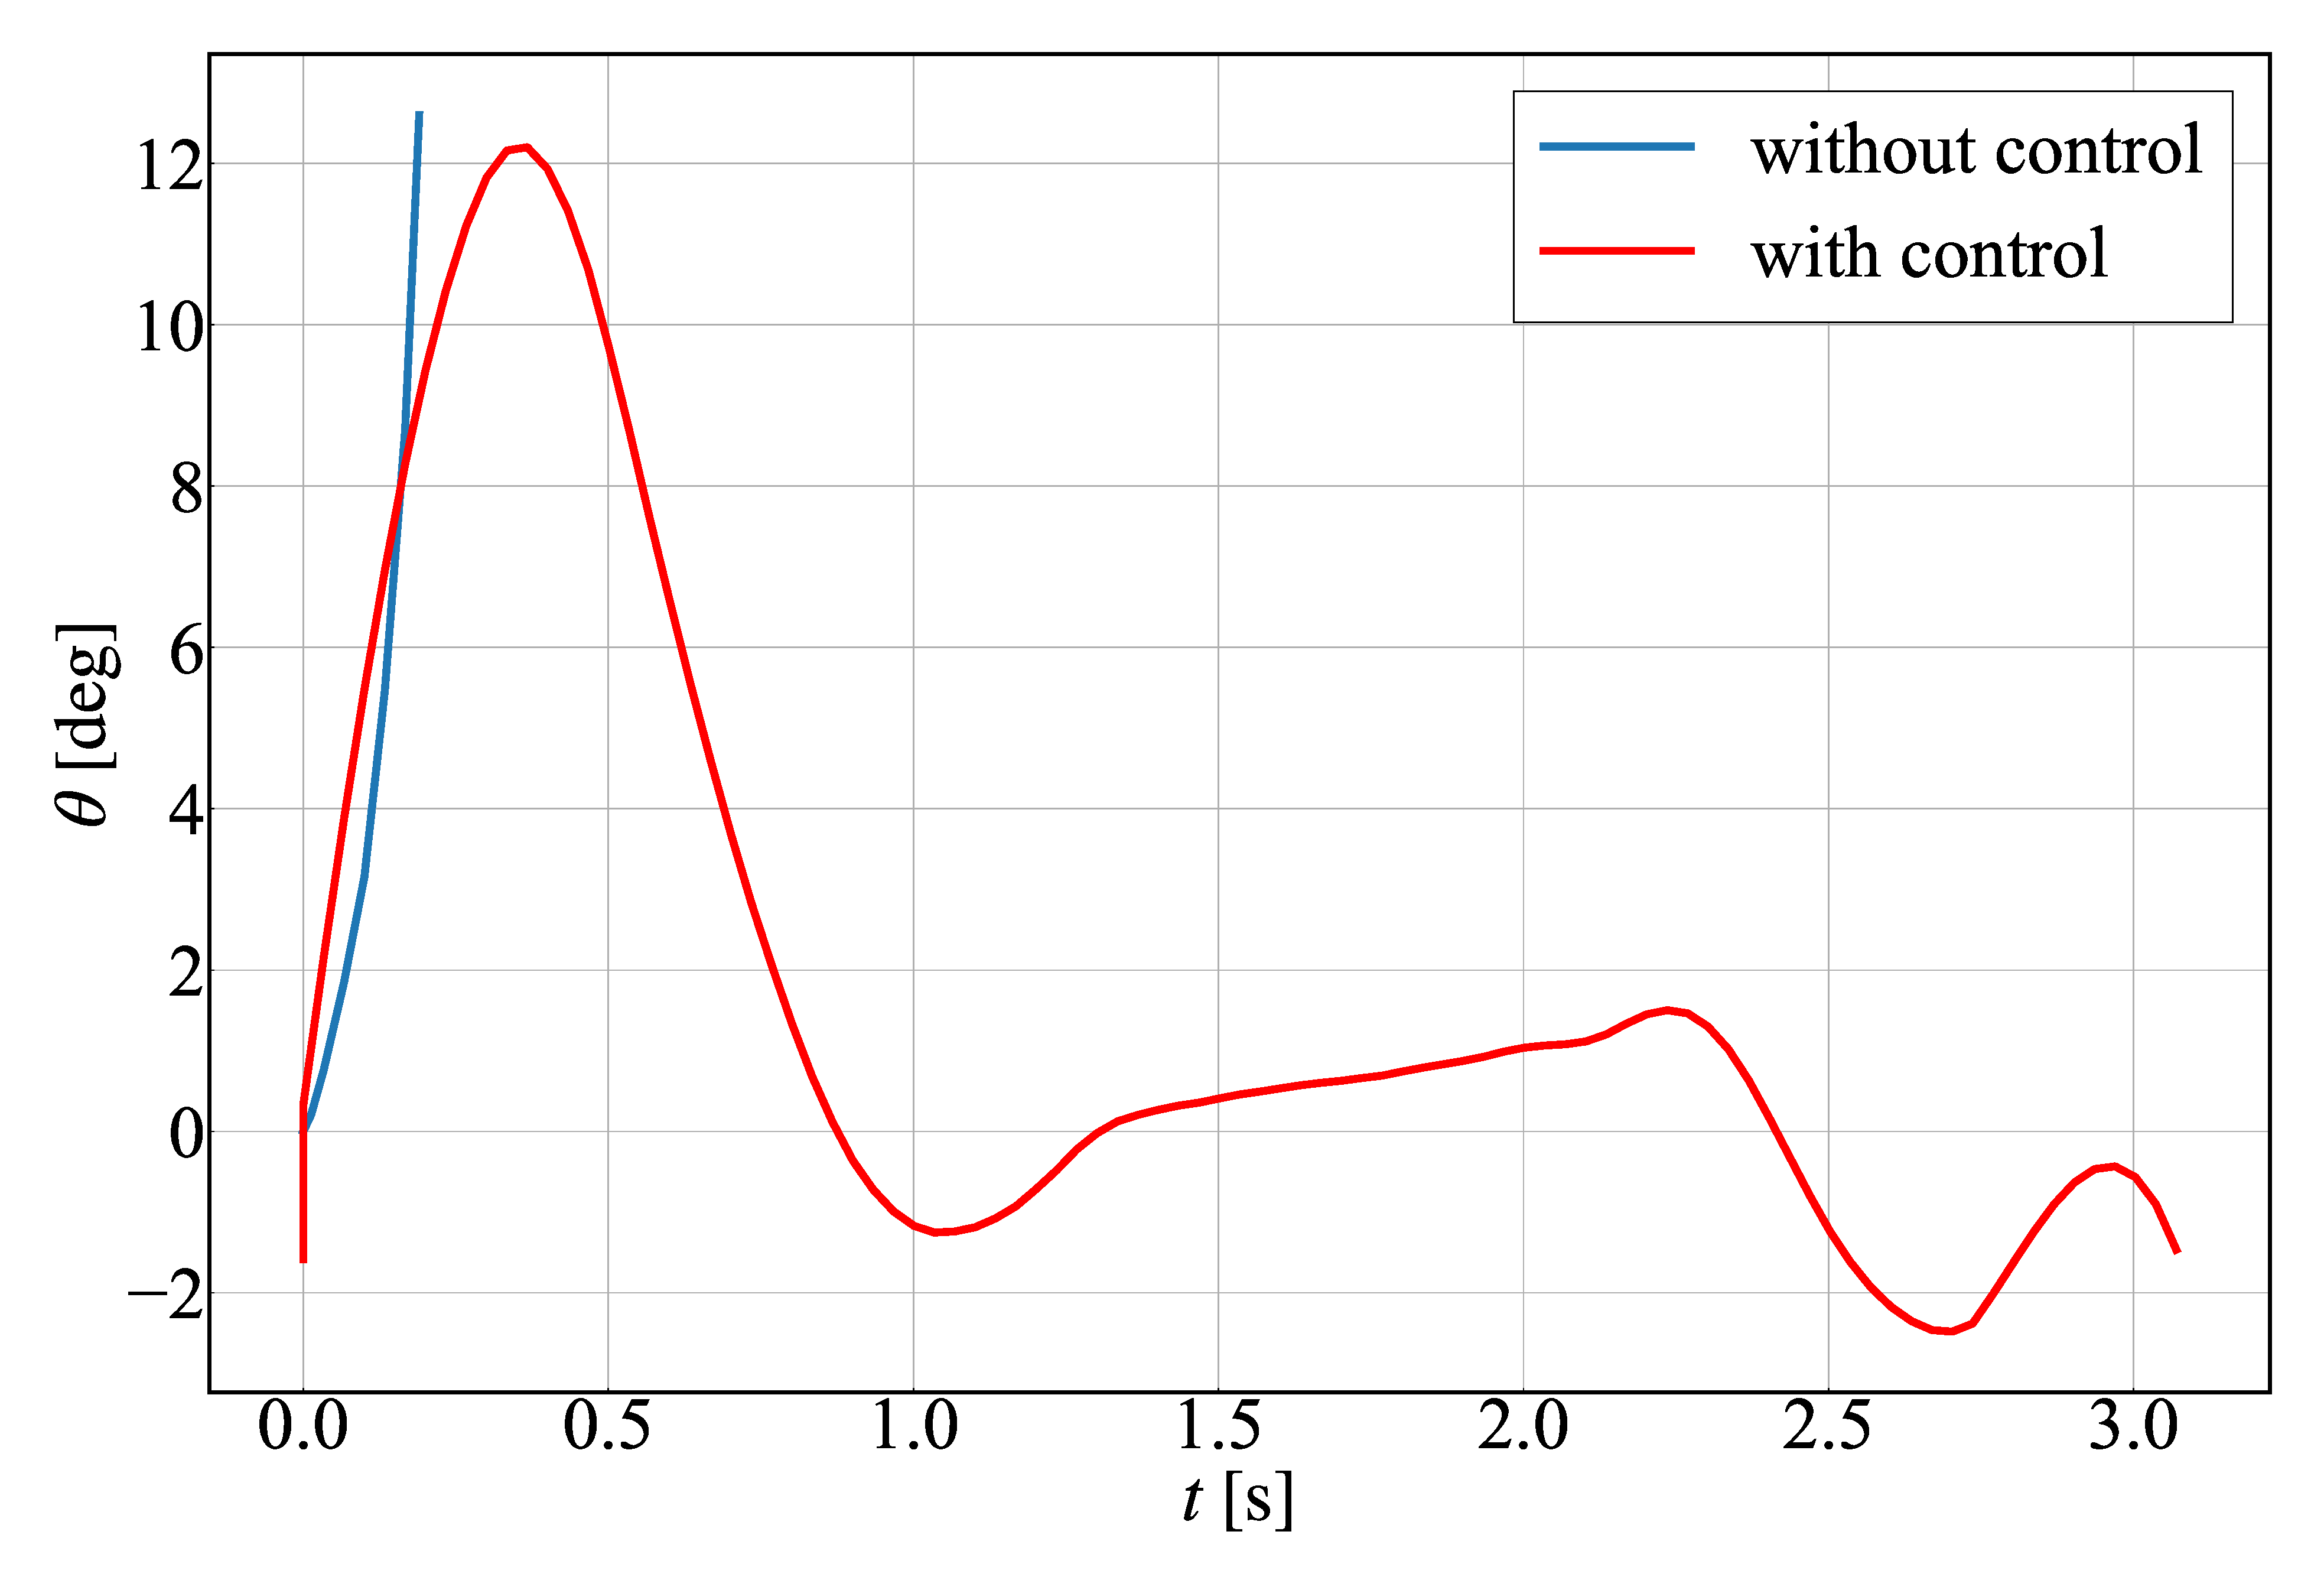
\includegraphics[width=0.8\columnwidth]{figures/angle-control.eps}
  \caption{Angle of object}
  \label{fig:angle}
\end{figure}
\reffig{angle}には,制御ありとなしの比較したときの角度のグラフを示す.横軸は時間$t$,縦軸は物体の初期姿勢からの角度のずれ\si{\degree}である.ここで,物体の角度は進行方向の逆向きを正とする.制御なしの場合の角度は設定された$\pm3$\si{\degree}の範囲外にあることがわかった.一方,制御ありの場合は,$t=0$~sから$t=0.5$~sまでは,物体の初期姿勢から12\si{\degree}傾いたものの,$t=0.5$~s以降,物体の初期姿勢からの角度差は0に近づき,$\pm1.8$\si{\degree}範囲内に収めることがわかった.よって,制御をかけることで,ロボット1段でも支持することができると言える.その他,急に動き出すときの大きい角度差に対して,今後ロボットに搭載されている加速度センサを利用して,フィードフォワード制御をかけることで,より安定に運搬できると考えられる.
\section{結言}
\labsec{conclusion}
本研究では,物体の重心付近まで乗り上げてロボットの体のみで支持できるロボット群を開発した.
そして実機実験の結果により,ロボットが他のロボットに乗り上げられること,移動部が移動するとき不安定な物体を支持できることが確認できた.
また,制御することで,より安定な協調運搬も確認できた..

\small
\bibliographystyle{osukalab}
\bibliography{main}

\clearpage
\end{document}
